\documentclass[12pt]{article}
\usepackage{geometry}                % See geometry.pdf to learn the layout options. There are lots.
\geometry{a4paper}    
\usepackage[german]{babel}               
\usepackage{graphicx}
\usepackage{amssymb}
\usepackage{amsthm}
\usepackage{epstopdf}
\usepackage[utf8]{inputenc}
\usepackage[usenames,dvipsnames]{color}
\usepackage[table]{xcolor}
\usepackage{hyperref}
\usepackage{eurosym}

\DeclareGraphicsRule{.tif}{png}{.png}{`convert #1 `dirname #1`/`basename #1 .tif`.png}

\theoremstyle{definition}
\newtheorem{example}{Example}

\newenvironment{explanation}{%
   \setlength{\parindent}{24pt}
   \itshape
   \color{blue}
}{}

%Dies kann -und sollte bei der Ausgangssituation anstelle der doppelten Backslashes verwendet werden! -MH
\newcommand*{\skippingparagraph}{\par\vspace{\baselineskip}\noindent}

\newcommand{\projectname}{ReceiptManager}
\newcommand{\productname}{ReceiptManager}
\newcommand{\projectleader}{J. Richtsfeld}
\newcommand{\documentstatus}{In Arbeit}
\newcommand{\version}{V. 1.0}

\begin{document}
\begin{titlepage}
\begin{flushright}

\includegraphics[scale=.5]{htlleondinglogo.png}
\end{flushright}



\vspace{10em}

\begin{center}
{\Huge Projektantrag} \\[3em]
{\LARGE \productname} \\[3em]
\end{center}

\begin{flushleft}
\begin{tabular}{|l|l|}
\hline
Projekt Name & \projectname \\ \hline
Projekt Leiter & \projectleader \\ \hline
Dokumenten Status & \documentstatus \\ \hline
Version & \version \\ \hline
\end{tabular}
\end{flushleft}

\end{titlepage}
\section*{Revisions}
\begin{tabular}{|l|l|l|}
\hline
\cellcolor[gray]{0.5}\textcolor{white}{Date} & \cellcolor[gray]{0.5}\textcolor{white}{Author} & \cellcolor[gray]{0.5}\textcolor{white}{Change} \\ \hline
16.09.2019&J.R./G.R./M.H./M.K.&Erste version \\ \hline
20.09.2019&J.R./G.R./M.H./M.K.&Projektziele überarbeitet \\ \hline
23.09.2019&J.R./G.R./M.H./M.K.&Rechtliches und Rahmenbedingungen \\ \hline
27.09.2019&J.R./G.R./M.H./M.K.&Projektantrag Korrektur und Finalisierung \\ \hline
\end{tabular}
\pagebreak
\tableofcontents
\pagebreak

\section{Einleitung}

Unser Projekt ist eine elektronische Belegsverwaltung, genannt ReceiptManager. Diese Software soll in einer Steuerberatungskanzlei die Arbeit für Steuerberater und Klienten erleichtern. Außerdem besteht ein großes Einsparungspotential, da die unötigen und stupiden Arbeiten der Rechnungsverwaltung wegfallen und durch unsere Software ersetzt werden. Desweitern wird es als Erweiterung für schon bestehende Buchhaltungssysteme, die keine digitale Belegverwaltung oder automatisches Einlesen von Rechnung anbieten, verwendet.
\pagebreak

\section{Ausgangssituation}

Aktuell müssen Klienten einer Steuerberatungskanzlei die Belege noch woechentlich bzw. monatlich zur Kanzlei bringen, damit die Buchhaltung erledigt werden kann.
\skippingparagraph
Danach müssen die Belege in Ordner abgelegt werden, diese Ordner werden dann in Wandschränke gebracht und alphabetisch und nach Jahr sortiert. Aktuell werden die Belegordner nach 5 Jahren aus den Schränken entfernt und in einen Lagerraum gebracht, dort sind sie wie in den Wandschränken sortiert und müssen noch weitere 2 Jahre aufgehoben werden. Ein großes Problem hierbei ist, der große Platzbedarf bei der Lagerung der Rechnungen, für die sogar eigene Kellerabteile gemietet werden.
\skippingparagraph
Durch die Buchhalter werden die essentiellen Werte (Rechnungsbetrag, Rechnungstyp, Steuersatz, usw.) der aktuellen Belege in die Buchhaltungssoftware über\-tragen, damit dann die Buchungen durchgeführt werden können und die Buchhaltung erledigt werden kann.
Derzeit verbringt ein Buchhalter etwa 20 Prozent seiner Zeit mit dem Verwalten und Auslesen von Rechnungen. Wenn ein Mitarbeiter im Monat um die 150 Stunden arbeitet, spart er sich dadurch 25 Stunden an Arbeitszeit. Außerdem wird weniger Platz für die Aufbewahrung der Rechnungen benötigt und dadurch können eventuell Mietkosten gespart.
\skippingparagraph
Aktuell gibt es zwei Firmen, Scopevisio und Parashift, die Komplettlösungen von der Buchhaltung bis zur automatischen Rechnungsverwaltung anbieten.
\skippingparagraph
Die Aktiengesellschaft Parashift wirbt stark mit deren Rechnungserkennungsalgorithmus, der sehr treffsicher sein sollte. Sie bieten diesen Service als eine API oder verbunden mit ihrer Software an. Diese Software liest komplett ohne manuelle Eingaben alle wichtigen Elemente aus einer Rechnu3ng oder einem Beleg, doch die Informationen können natürlich darauffolgend bearbeitet werden, wenn es nötig ist.
\skippingparagraph
Die Scopevisio AG bietet eine Komplettlösung an und setzt auch auf eine KI, doch verlässt sich nach der Erkennung auf den Steuerberater, der diese Daten überprüfen muss. Dies hat den Nachteil, dass es zu Lasten von dem Steuerberater fällt, jedoch sorgt dies für eine 100 Prozentige Trefferquote.
\skippingparagraph
Unsere Software soll als Erweiterung für Buchhaltungssysteme dienen, die den Teil der Rechnungsverwaltung und Rechnungseinlesen nicht anbieten. So muss der Steuerberater nicht das ihm bekannte Buchhaltungssystem wechseln, wenn er diese Erweiterungen haben möchte.
\par
\pagebreak

\section{Allgemeine Bedinungen und Einschränkungen}
Unsere System muss mit folgenden Problemen umgehen können: 
\skippingparagraph
Die Rechnungen müssen laut der Bundesabgabenordnung (BAO) mindestens 7 Jahre aufgehoben werden, wobei es keine Beschränkung auf die Form der Speicherung gibt.
\skippingparagraph
Die Datenbank muss täglich gesichert werden, damit im Falle eines Systemausfalls oder -schadens keine Daten verloren gehen.
\skippingparagraph
Jeder Nutzer muss sich authentifizieren, damit die sensiblen Daten der Rechnungen geschützt werden können.
Ein Mobileclient wird benötigt, um auf die Kamera des Mobiltelfons zugreifen zu können um so direkt den Beleg/ die Rechnung zu erfassen. Um den ReceiptManager auch am PC verwenden zu können oder Fotos in größeren Mengen zu übertragen, wird ein Webclient benötigt.
\skippingparagraph
Der Steuerberater soll möglich sein, schnell Belege und die dazu relevanten Informationen zu finden, ohne dabei mehrere Ordner mit Rechnungen durchforsten zu müssen.
\skippingparagraph
Desweitern soll die Verantwortung für die Richtigkeit der Rechnungswerte beim Steuerberater bleiben, um den Aufwand für den Klienten zu minimalisieren.
\par
\pagebreak

\section{Projektziele und Systemkonzepte}
Die Projektziele werden wie folgt zusammengefasst:

\subsection{Benutzeroberfläche Steuerberater}
Die Rechnungen können nach Klienten gruppiert, nach Attributen sortiert oder nach Attributen sortiert werden. Sortierattribute sind das Rechnungsdatum, der Betrag und das Hochladedatum. 
In einem Rechnungseingang sind die Mandanten und die Anzahl ihrer zur Bestätigung ausstehenden Rechnungen aufgelistet.
\par
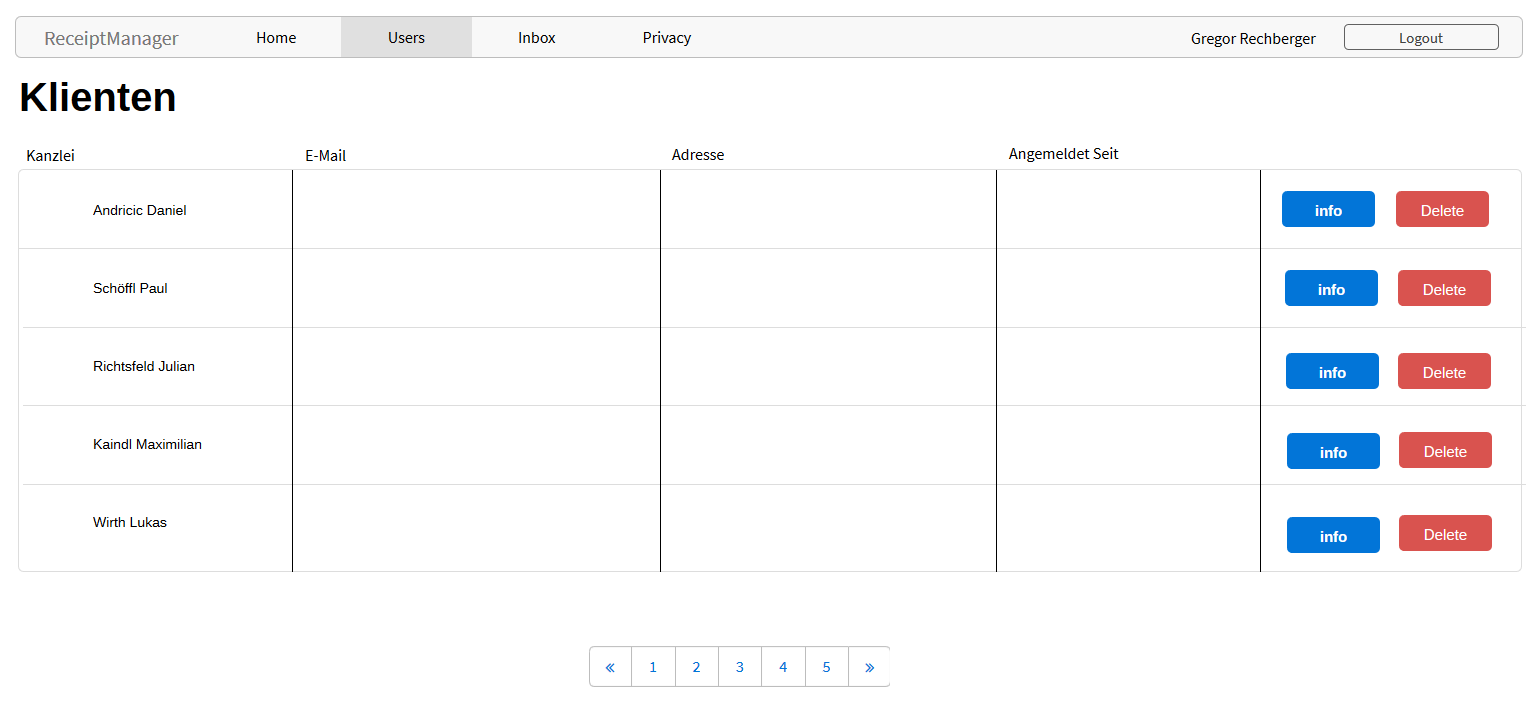
\includegraphics[width=\linewidth]{MandantenListeConcept}

\pagebreak
\noindent Beim Auswählen eines Mandantes wird auf eine Liste seiner eingegangenen Rechnungen weitergeleitet, wo dann weiters einzelne Rechnungen korrigiert und in das System aufgenommen werden können.
\par

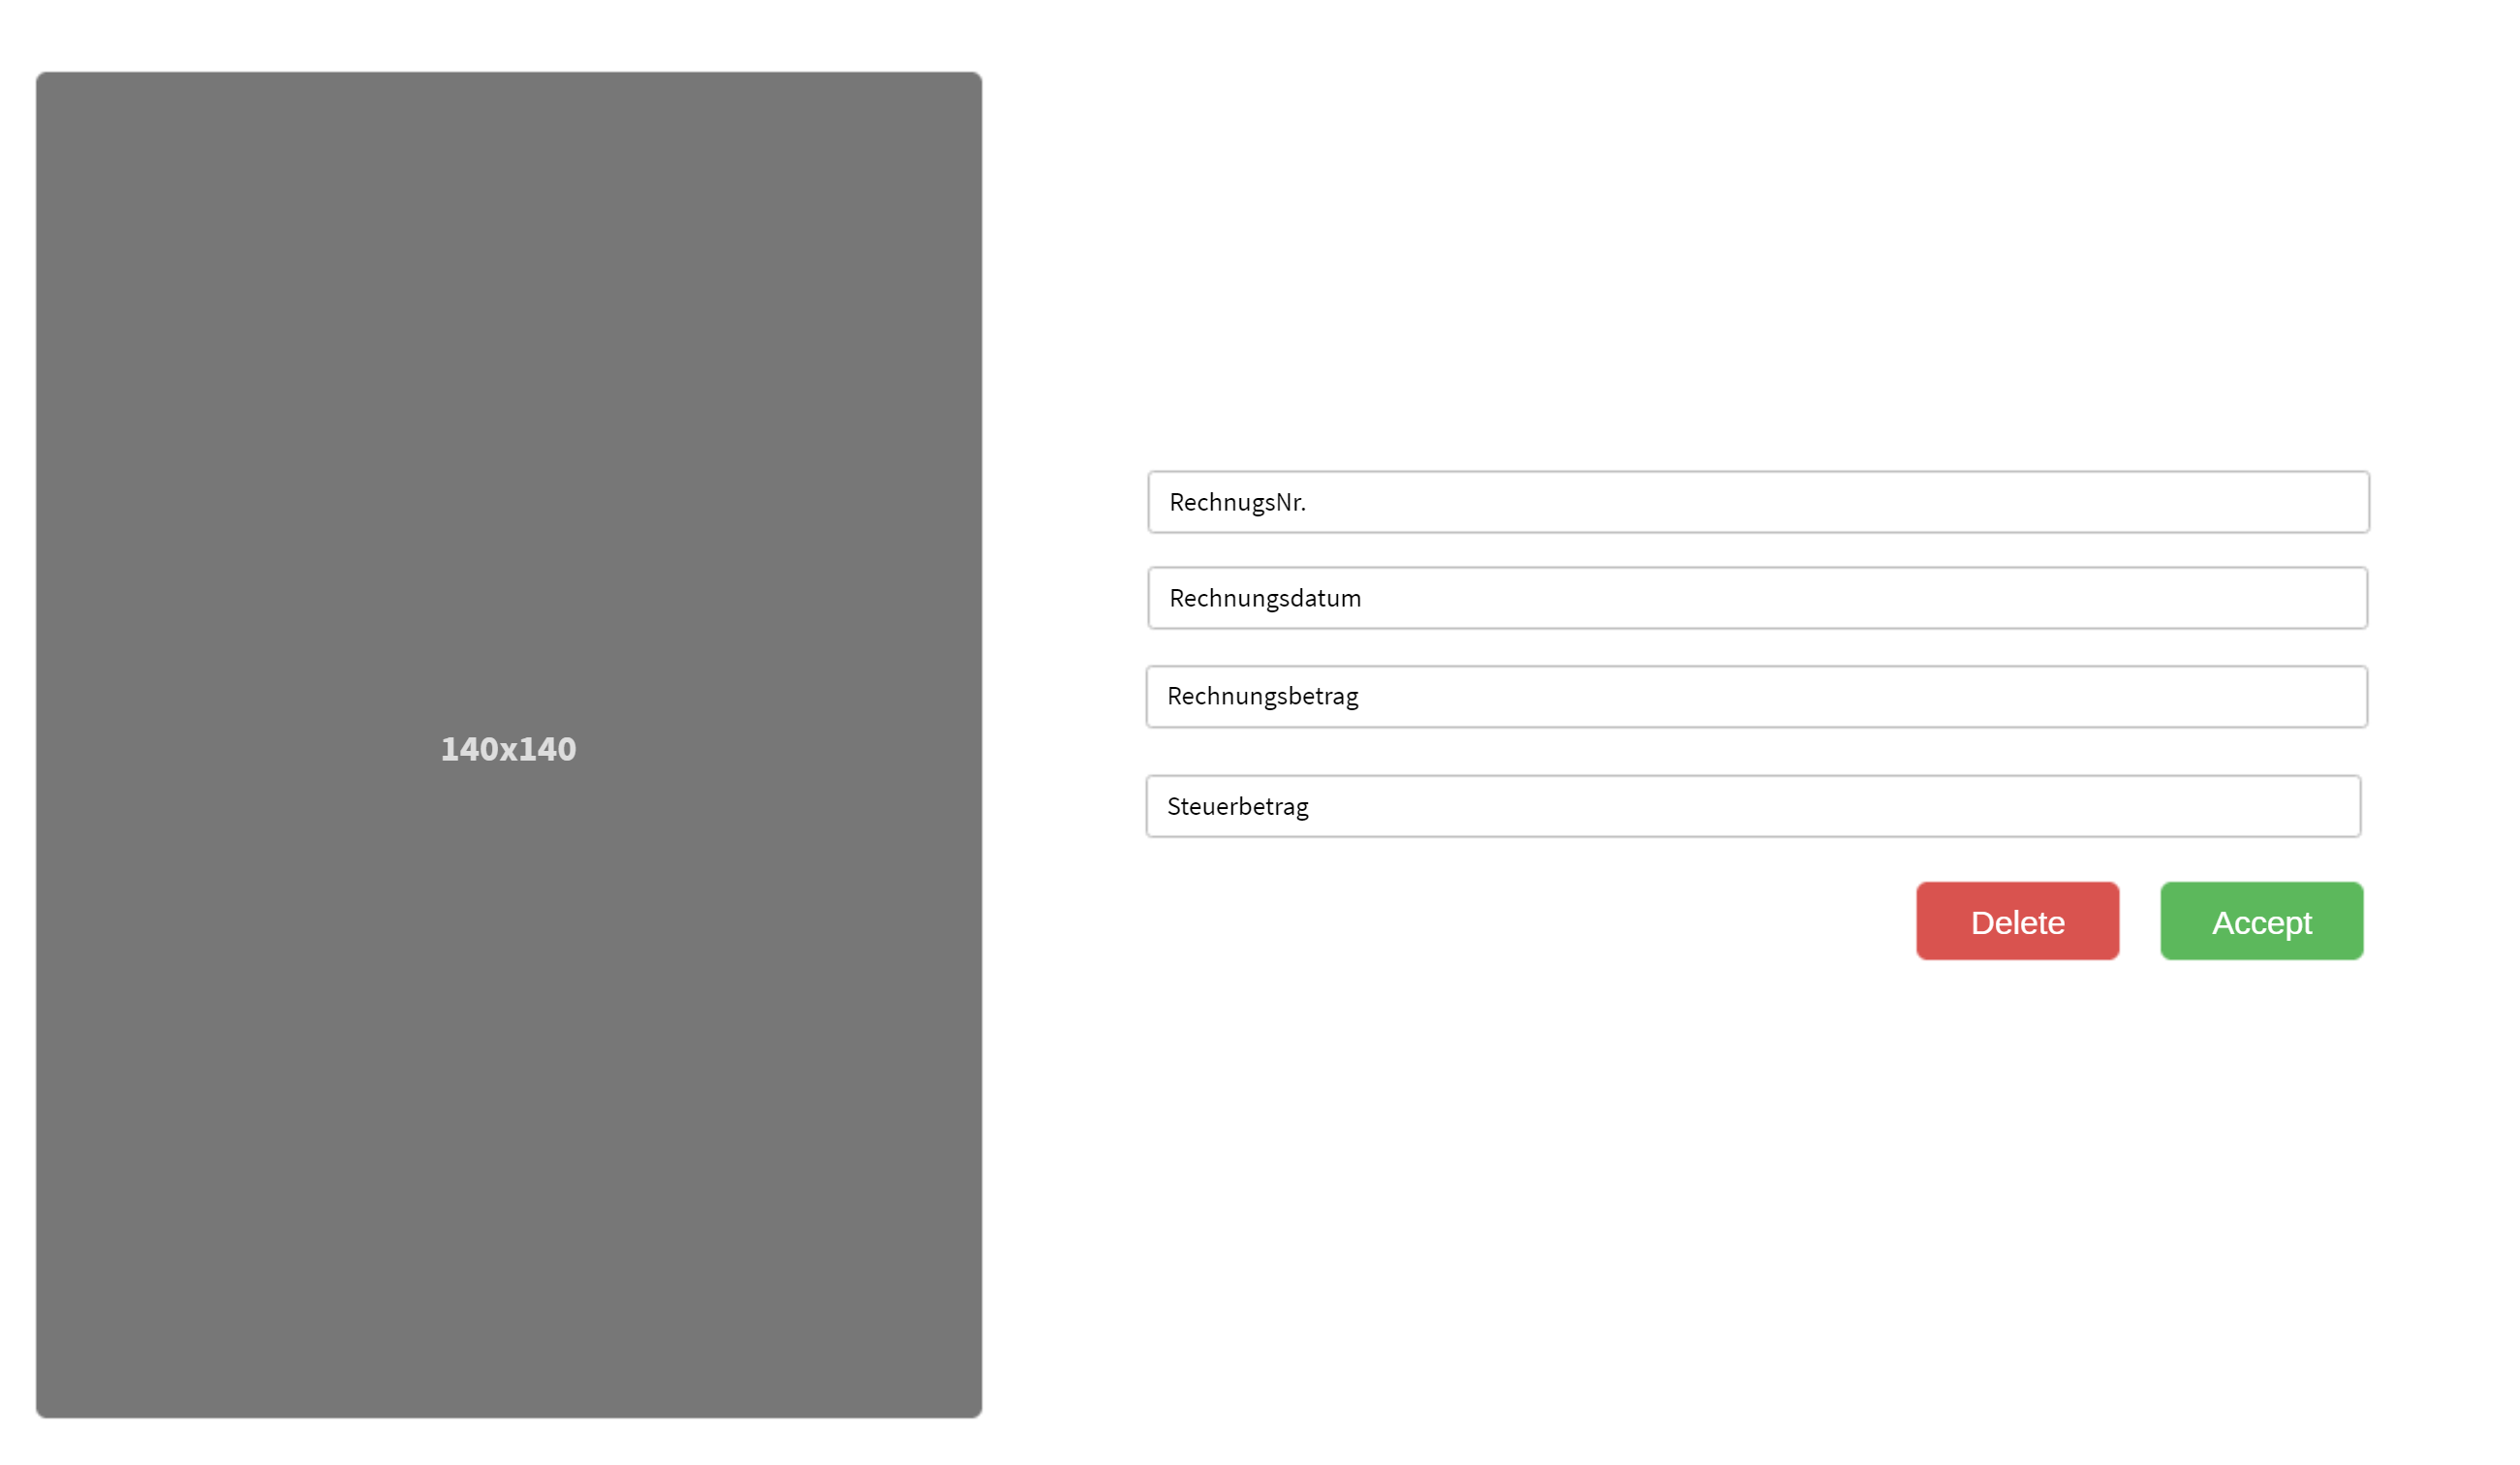
\includegraphics[width=\linewidth]{SingleReceiptReview}

\noindent Innerhalb eines Jahres können die Rechnungen nach Datum und Betrag sortiert werden, um dem Steuerberater das Suchen der Rechnungen/Belege möglichst einfach und schnell zu gestalten.
\par

\pagebreak
\subsection{Benutzeroberfläche Klient}
Ein großer Fokus liegt bei dem Projekt auf einer Mobilapp für den Klienten. Die Kamera und kompakte Bauart eines Smartphones ermöglicht schnelle Schnappschüsse und benötigt keinen Scanner.

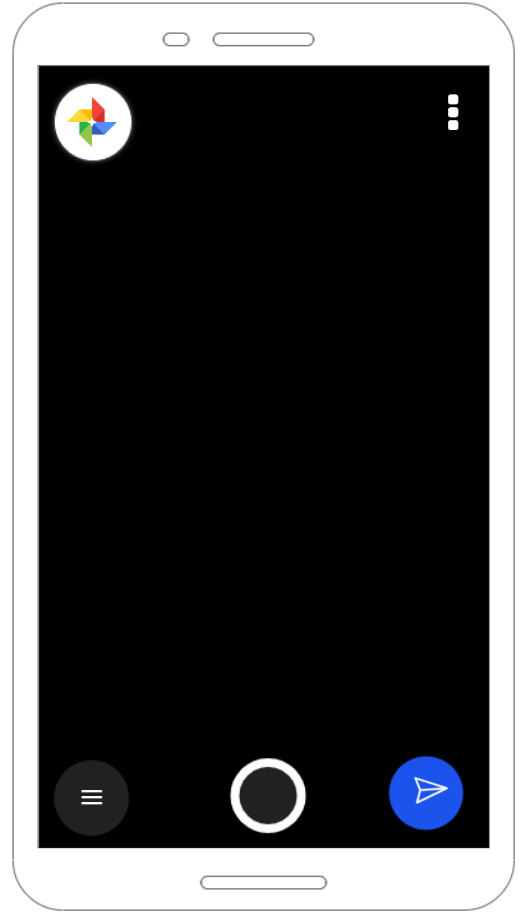
\includegraphics[scale=0.5]{MobileSnapshotReceiptConcept}

\pagebreak
\subsection{Backend}
Das Backend soll auf zwei Teile aufgeteilt werden. Zum einen das OCR- System als Microservice und zum anderen das Hauptbackend zum Speichern und Verwalten der Belege.
\skippingparagraph
Beim Frontend wird für die Klienten eine Web App bzw. Mobileapp angeboten. Der Steuerberater sieht die Admin-Oberfläche nur in der Webapp da, kein Bedarf besteht dies in einer Mobileapp zu realisieren.

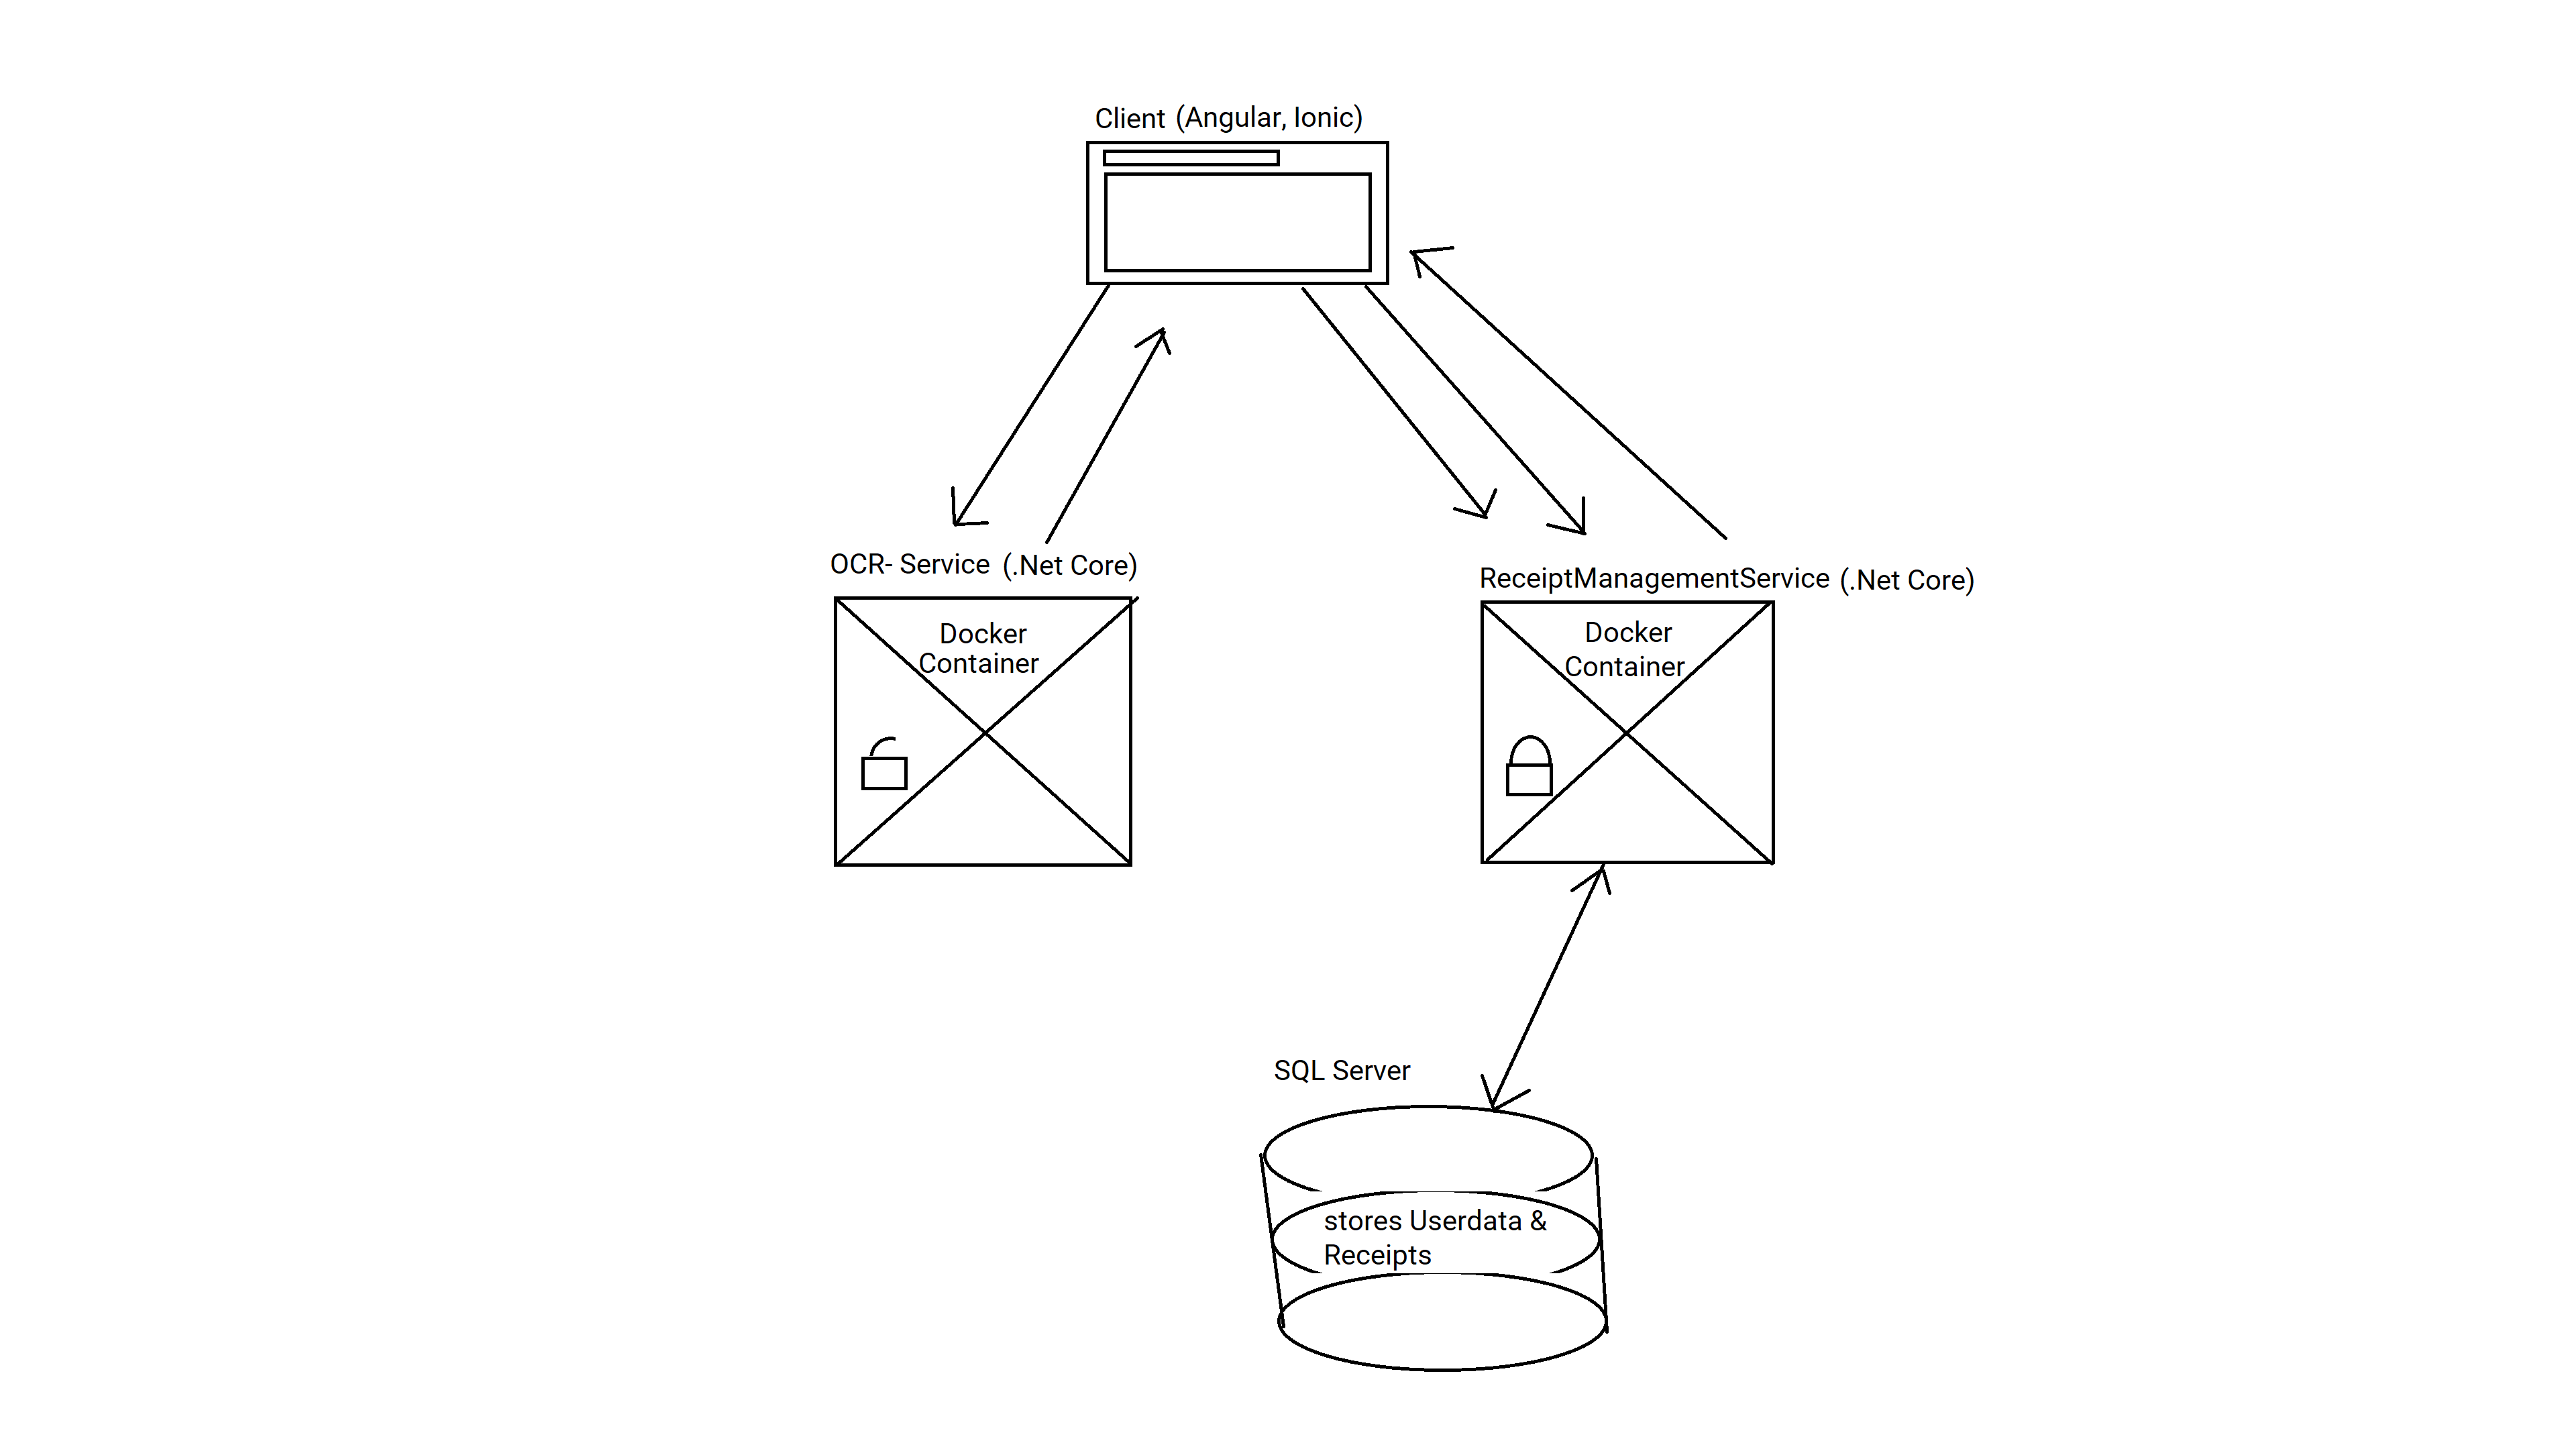
\includegraphics[width=\linewidth,trim=130mm 10mm 100mm 10mm, clip]{SystemConcept}
\pagebreak


\section{Chancen und Risken}

\subsection{Vorteile und Chancen durch und von unsere Software}

Der Klient kann sich durch unsere Software Zeit und daher Geld sparen, da er keine Zeit mehr verschwenden muss, um die Rechnungen bei sich in Ordner einzusortieren und diese dann zum Steuerberater zu bringen.\\ \\
Die Verwaltung der Rechnungen wird einfacher und übersichtlicher, da das Suchen der Rechnungen in Ordner wegfällt und durch einfaches und schnelles Suchen in unserer Anwendung ersetzt wird.\\ \\
Ein großer Vorteil ist die Ersparniss vom Arbeitszeit, da ein Buchhalter etwa 20 Prozent seiner Zeit mit dem Verwalten und Auslesen von Rechnungen verbringt. Bei einem Brutto-Monatsgehalt von \EUR{3000}, werden im Jahr etwa \EUR{8000} und im Monat \EUR{600} pro Mitarbeiter eingespart. Außerdem steigert unsere Anwendung die Produktivität der Buchhalter da sie sich nicht mehr mit den stupiden Arbeiten der Verwaltung auseinander setzen müssen.\\



\subsection{Risiken unserer Software}

Folgende Risiken müssen beachtet werden:
\begin{itemize}
\item Verlust von Belegen, die sensible Informationen enthalten, da es beim Übertragen der Daten zu Fehlern kommen kann.
\item Durch falsch eingegebene von Informationen durch den Steuerberater, könnten inkonsistente Datenbestände entstehen.
\end{itemize}

\pagebreak

\section{Planung}

\subsection{Teammitglieder}

\begin{itemize}
\item Teamleiter: Julian Richtsfeld
\item Entwickler für Benutzeroberfläche: Maximilian Kaindl
\item Entwickler für Web- und Mobilklienten: Matthias Hofmarcher
\item Entwickler für OCR- und Parsercontainer für automatische Beleginformationserkennung: Gregor Rechberger
\item Entwickler für Backend: Julian Richtsfeld
\end{itemize}

\subsection{Meilensteine}

\begin{tabular}{|l|l|}
\hline
\cellcolor[gray]{0.5}\textcolor{white}{Date} & \cellcolor[gray]{0.5}\textcolor{white}{Meilenstein} \\ \hline
20.12.2019&Authentifizierung mit JSON-Webtoken und Identity Server 4\\ \hline
28.02.2020&Server Prototyp als Api-Endpunkt lauffähig \\ \hline
03.04.2020&Web-Client Prototyp lauffähig \\ \hline
24.04.2020&OCR-Prototyp abgeschlossen \\ \hline
29.05.2020&Mobile-Client-Prototyp lauffähig\\ \hline
26.06.2020&Lauffähiger Receipt-Manager Prototyp\\ \hline
\end{tabular}

\subsection{Benoetigte Ressourcen}

\begin{itemize}
\item Server (Eigenbau oder Cloud)
\item OCR-Software Lizenz
\end{itemize}

\subsection{Projektdauer}
Das Projekt beginnt mit 20.09.2019 und endet mit dem Ende des Schuljahres 2019/20. Der erste Prototyp wird Mitte November zur Verfuegung stehen. Die Implementierung beginnt mit Abschluss des Prototyps. Die groeßeren Arbeitspakete sind die Entwicklungs des Front -und Backends und die Einbindung einer OCR-Software. Unsere Ziele schaetzen wir durchaus realistisch ein und gehen von einer fristgerechten Umsetzung aus.

\end{document}  